
\section{Teksto pavyzdžiai}

\par Vienas paragrafas

\par Antras paragrafas

\par Sąrašas:

\begin{itemize}
  \item reikia A;
  \item reikia B;
  \item nereikia C.
\end{itemize}

\par Formulė:

\par \begin{equation}
  \text{veiksnumas} = \frac{\text{MTBF} - \text{MTTR}}{\text{MTBF}}
\end{equation}

\par Lentelė:

\begingroup
\fontsize{12pt}{14pt}\selectfont
\begin{tabularx}{0.93\textwidth}{ l l p{6.5cm} }
  Data  & Tekstas \\
  \hline
  2006 Rugsėjo 1 d. & Lorem ipsum \\
  \hline
  2012 Rugsėjo 19 d. & dolor sit amet \\
  \hline
\end{tabularx}
\endgroup
\vskip 1cm


\section{Grafiniai pavyzdžiai}

\par Diagrama:

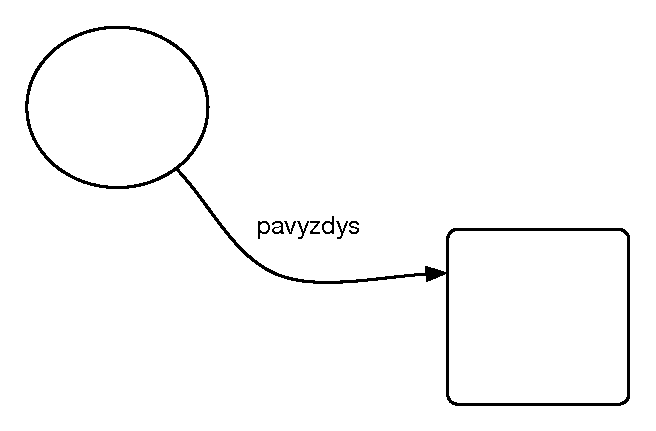
\includegraphics[angle=0,scale=0.75]{assets/diagram.eps}

\par Iliustracija:

\begin{figure}[H]
  \centering
  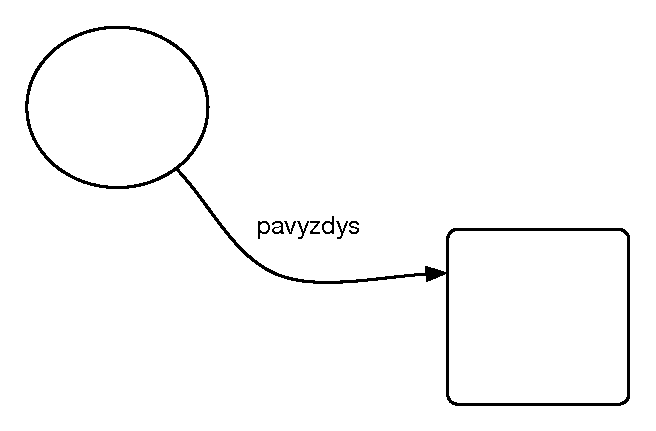
\includegraphics[scale=0.4]{assets/diagram.eps}
  \caption{Iliustracijos pavadinimas.}
\end{figure}
